En esta sección se detalla la implementación de cada paso realizado para la limpieza de los datos. Este proceso precede a la fase de adquisición de los datos y se enfoca en el tratamiento de numerosos documentos de texto. La limpieza de texto incluye diversas tareas necesarias para procesar los archivos de comentarios adquiridos, tales como la conversión y el tratamiento de los formatos obtenidos de sus respectivas fuentes. Esto implica eliminar todo el contenido innecesario que rodea al texto, asegurando así su preprocesamiento y utilidad para el entrenamiento de modelos. El resultado es un conjunto de archivos útil, limpio, bien distribuido y en el formato requerido. Dado que las tareas de limpieza son numerosas, esta sección se ha dividido en dos partes representadas por dos carpetas, cada una con un propósito específico, las mismas se describen a continuación:

La carpeta limpiezadataset almacena dos archivos, el archivo encargado de la limpieza de datos es el siguiente:

\begin{itemize}

\item limpiar\_datos.py: Este archivo se encarga de los aspectos específicos de limpieza para cada fuente de información. Por ejemplo, la limpieza de datos extraídos de la red social Facebook no será la misma que la de datos provenientes de la red social WhatsApp. Las funciones y detalles de este archivo se ilustran en la figura \ref{fig:uml1}.

\begin{figure}[h!]
	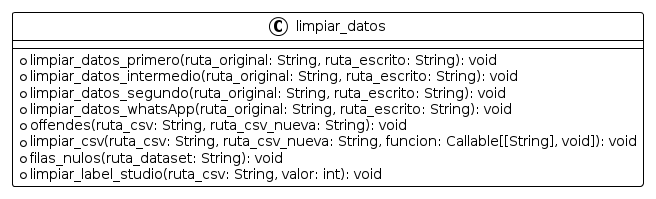
\includegraphics[width=0.65\textwidth]{capitulo5/figuras/fig1.png}
	\caption[Diagrama de clase del archivo limpiar\_datos]{Diagrama de clase del archivo limpiar\_datos
		\\\textit{Fuente: Elaboracion Propia}}
	\label{fig:uml1}
\end{figure}

\end{itemize}

%\textbf{Formato y Encadenamiento de Información}

La carpeta gestionarchivos contiene los archivos manejo\_archivos.py y convertir\_formato.py cada uno es importante para el uso de las funciones del archivo limpiar\_datos.py a continuacion se describen estos archivos:

\begin{itemize}

\item manejo\_archivos.py: Este archivo se encarga de la creación, copia, recorrido y vaciado de archivos en diferentes formatos. Para más detalles, consulte la figura \ref{fig:uml3}.

\begin{figure}[h!]
	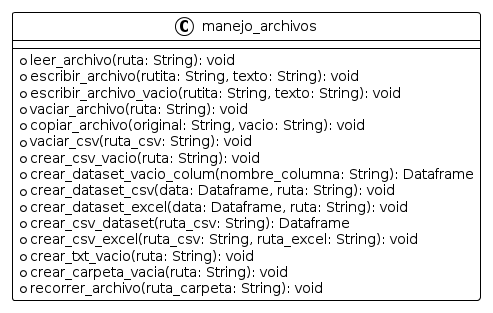
\includegraphics[width=0.65\textwidth]{capitulo5/figuras/fig3.png}
	\caption[Diagrama de clase del archivo manejo\_archivos]{Diagrama de clase del archivo manejo\_archivos
		\\\textit{Fuente: Elaboracion Propia}}
	\label{fig:uml3}
\end{figure}


\item convertir\_formato.py: Este archivo se ocupa de agrupar información de múltiples archivos para hacer uso de forma masiva de las funciones de limpieza definidas en el archivo limpiar\_datos.py, además de manejar el formato de los mismos cuando sea necesario. Para más detalles, consulte la figura \ref{fig:uml4}.

\begin{figure}[h!]
	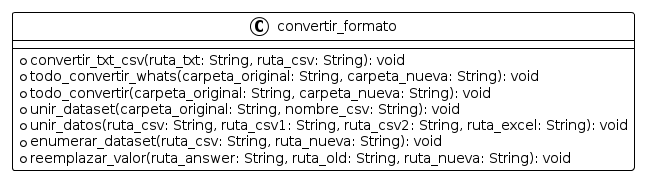
\includegraphics[width=0.8\textwidth]{capitulo5/figuras/fig4.png}
	\caption[Diagrama de clase del archivo convertir\_formato]{Diagrama de clase del archivo convertir\_formato
		\\\textit{Fuente: Elaboracion Propia}}
	\label{fig:uml4}
\end{figure}

\end{itemize}

Es importante recordar que el preprocesamiento de datos varía según la fuente de los datos. Para más detalles sobre el proceso de limpieza de los datos provenientes de Facebook, consulte la figura \ref{fig:um12} (diagrama de actividades de Facebook) y el proceso de limpieza de datos provenientes de WhatsApp se puede apreciar en la figura \ref{fig:um13}(diagrama de actividades de Whatsapp).

\begin{figure}[h!]
	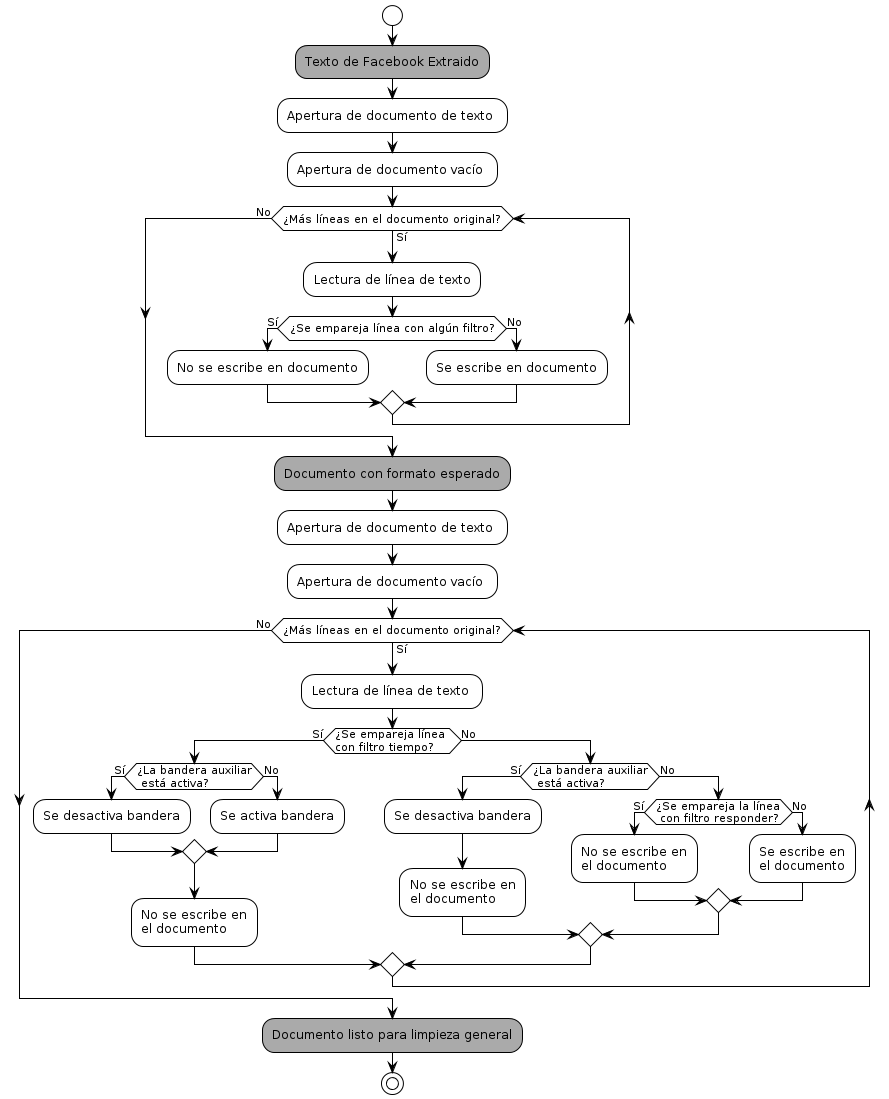
\includegraphics[width=1\textwidth]{capitulo5/figuras/prueba.png}
	\caption[Diagrama de actividades limpieza datos facebook]{Diagrama de actividades limpieza datos facebook
		\\\textit{Fuente: Elaboracion Propia}}
	\label{fig:um12}
\end{figure}

\begin{figure}[h!]
	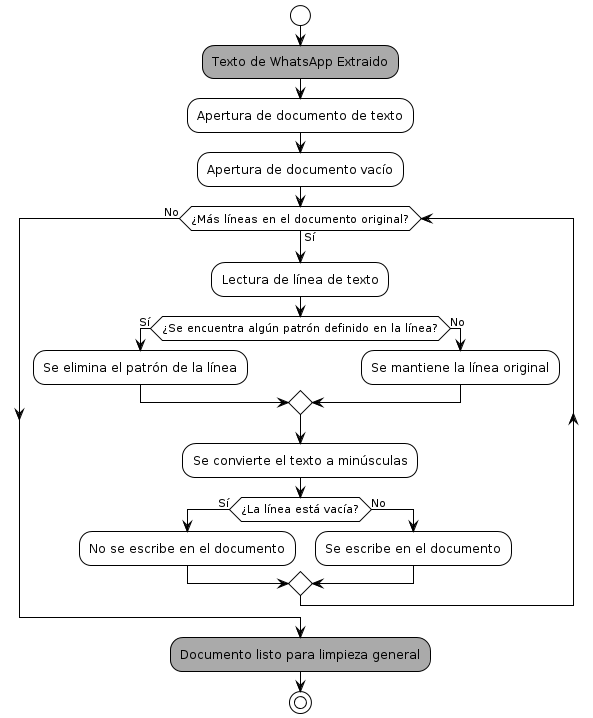
\includegraphics[width=0.7\textwidth]{capitulo5/figuras/part3.png}
	\caption[Diagrama de actividades limpieza datos whatsapp]{Diagrama de actividades limpieza datos whatsapp
		\\\textit{Fuente: Elaboracion Propia}}
	\label{fig:um13}
\end{figure}


\clearpage
